\documentclass[12pt,letterpaper]{article}
\usepackage{amsmath,amsthm,amsfonts,amssymb,amscd}
\usepackage{fullpage}
\usepackage{lastpage}
\usepackage{enumerate}
\usepackage{fancyhdr}
\usepackage{mathrsfs}
\usepackage{mathtools}
\usepackage{mdframed}
\usepackage{tikz}
\usepackage{float}
\usetikzlibrary{calc,trees,positioning,arrows,fit,shapes,calc}
\usepackage[margin=3cm]{geometry}
\setlength{\parindent}{0.0in}
\setlength{\parskip}{0.05in}

% Edit these as appropriate
\newcommand\course{CSCI 0220}
\newcommand\semester{Summer 2021}     % <-- current semester
\newcommand\definition{\textbf{Definition: }}
\newcommand\proposition{\textbf{Proposition: }}
\newcommand{\defeq}{\vcentcolon=}
\newcommand{\example}{\textit{Example: }}
\newcommand{\claim}{\underline{Claim:} }
\newcommand{\idea}{\textit{Idea:} }

% Common Commands
\newcommand\N{\mathbb N}
\newcommand\Z{\mathbb Z}
\newcommand\R{\mathbb R}
\newcommand\Q{\mathbb Q}
\newcommand\lcm{\operatorname{lcm}}
\newcommand\setbuilder[2]{\ensuremath{\left\{#1\;\middle|\;#2\right\}}}
\newcommand\E{\operatorname{E}}
\newcommand\V{\operatorname{V}}
\newcommand\Pow{\ensuremath{\operatorname{\mathcal{P}}}}

\newenvironment{answer}[1]{
  \subsubsection*{Problem \hwnum.#1}
}{\newpage}

\pagestyle{fancyplain}
\headheight 35pt
\lhead{\course}
\chead{\textbf{\Large Midterm Review Guide}}
\rhead{\semester}
\headsep 10pt

\begin{document}

\section{Disclaimer}

The TAs do not know what is on the midterm. The following is our guide for what we believe will be helpful in preparation. Additionally, the example proofs we provide in this review guide may be informal, or stripped to their bare bones. They strive to convey an idea, but are not necessarily paragons of perfect proofs. We suggest looking at the website or the homework solutions for polished proofs.

\section{Proof Techniques}

Here are some useful proof strategies.

    \subsection{Direct Proof}
    
    Given statements implies conclusion.
    
    \begin{mdframed}
    \claim The product of two odd numbers is odd,
    
    What we know:
    An odd number $n = 2k + 1$ for some $k \in \Z$.
    
    \[
    (2a+1)(2b+1) = 4ab + 2a + 2b + 1 = 2\underbrace{(2ab + a + b)}_{k \in \Z} + 1 = 2k+1.
    \]
    \end{mdframed}
    
    \subsection{Contradiction}
    
    Say we have some proposition $T$ that we are tyring to prove. Here is how we can  prove it by contradiction:
      \begin{enumerate}
        \item Assume $T$ is not true.
        \item Given $T$ is false, use a direct proof to obtain a contradiction.
        \item Since $T$ being false leads us to a contradiction, $T$ must be true.
      \end{enumerate}
      
    Often $T$ is of the form ``If $p$ then $q$." In this case, assume that $p$ is true and $q$ is false to reach a contradiction. Often, this contradiction will be of the form ``If $p$ is true and $q$ is false then $p$ is false. This conclusion is a contradiction as $p$ cannot both be true and false. 
    
    \begin{mdframed}
    For example 
    $$ \text{If }\underbrace{n^2 \text{ is even}}_{p} \text{ then } \underbrace{n \text{ is even.}}_{q}$$


    \begin{proof} Assume for sake of contradiction that $n^2$ is even but $n$ is odd. Since $n$ is odd, $n = 2k+1$ for some $k \in \Z$.

      So $n^2 = (2k+1)(2k+1) = 4k^2 + 4k + 1 = 2(2k^2 + 2k) + 1 = 2m+1$.

      Where $m =  2k^2 + 2k$.

      Since $m$ is an integer, $n^2$ is odd. This is a contradiction since $n^2$ is even, and therefore if $n^2$ is even then $n$ must also be even.
    \end{proof}
    
    \end{mdframed}
      
    \begin{mdframed}
        Consider a set $A = \{a_1,...,a_n\}$ with cardinality $n$.
        
        Consider $f:P(A) \rightarrow \{0,1\}^n$ where $f(X) = s_1s_2...s_n$ and $s_i = 1$ if $x_i \in X$ and $s_i = 0$ if $x_i \not\in X$. 
        
        \claim If $f(X_1) = f(X_2)$ then $X_1 = X_2$. 
                
        \begin{proof}
        Assume for sake of contradiction that $f(X_1) = f(X_2)$ but $X_1 \not= X_2$. Since $X_1 \not= X_2$, there must be some element in one set but not the other. Assume without loss of generality that $a_i \in X_1$ and $a_i \not\in X_2$. Then $f(X_1)$ will have a 1 at position $i$ but $f(X_2)$ will have a 0 at position $i$. This is a contradiction as we began by assuming that $f(X_1) = f(X_2)$. 
        \end{proof}
        
        \idea \textit{Can you see how this could have been done as a direct proof?}
    \end{mdframed}
    
    \subsection{Proof by Cases}
        
    \begin{mdframed}
    \claim There exists $x,y$ irrational such that $x^y$ is rational.
    
   \begin{proof}
    
    Consider $z = \sqrt{2}^{\sqrt{2}}$.
    
    \textbf{Case 1:} $z$ is rational. Let $x = y = \sqrt{2}$ then we are done.
    
    \textbf{Case 2:} $z$ is irrational. Then let $x = z$ and $y = \sqrt{2}$ and we get
    
    \[\sqrt{2}^{\sqrt{2}*\sqrt{2}} = \sqrt{2}^2 = 2\]
    \end{proof}
    \end{mdframed}
    
    \subsection{Counterexample}
    
    Counterexamples help us prove that something is not true.

      For example, suppose Kristy makes the claim that if $xy$ is rational then $x$ and $y$ are rational.

      Kareem can disprove her claim by coming up with a counterexample. For example, if $x = \sqrt{2}$ and $y = \sqrt{2}$, then $xy = 2$, which is rational. 

      However, you \textbf{cannot} prove a claim by showing one example of it. Kareem has not proven that $x$ and $y$ are irrational, he has just shown that they are not always rational.

      For example, the claim ``all CS22 students like donuts" can be disproved by finding a student who does not like donuts. Finding this counterexample, however, will not prove that no students like donuts.
      
      
    \begin{mdframed}
    \claim $\Pow{(A\cup B)} \not= \Pow{(A)}\cup \Pow{(B)}$
    \begin{proof}

		Consider $A = \{1\}$ and $B = \{2\}$. 

		Then $\{1,2\} \in \Pow{(A\cup B)}$ but $\{1,2\} \not\in \Pow{(A)}\cup \Pow{(B)}$.
    \end{proof}    
    \end{mdframed}
    \subsection{Proof by Element Method}
    
	How do you prove that two sets $A$ and $B$ satisfy $A = B$? First, you can show that $A \subseteq B$ and then you show that $B \subseteq A$. If every element in $A$ is also an element in $B$ and every element in $B$ is also an element of $A$, then $A$ must equal $B$. 

	To show that $A \subseteq B$ you consider an arbitrary element in $A$ and show it is also in $B$. 

\renewcommand{\iff}{\textrm{IFF}}

		\begin{mdframed}
		\claim $\Pow{(A\cap B)} = \Pow{(A)}\cap \Pow{(B)}$
		\begin{proof}
		\begin{align*}
		x \in \Pow{(A\cap B)}
		\iff & x \subseteq A \cap B \\
		\iff & x \subseteq A \text{ and } x \subseteq B \\
		\iff & x \in \Pow{(A)} \text{ and } x \in \Pow{(B)} \\
		\iff & x \in \Pow{(A)}\cap \Pow{(B)}
		\end{align*}
		\end{proof}		
		\end{mdframed}
    
    \subsection{Bijective Proof}
    
    Example provided later. (Put together proofs for injectivity and surjectivity further down in this sheet, and then add conclusion.)
    
    \subsection{Bidirectional Proof}
    
    If a claim is of the form ``A if and only if B," it is enough to prove both ``if A, then B" and ``if B, then A".
    
    \subsection{Inductive Proof}
    
    More detail later.


\section{Logic}

Here's information about logic.

    \subsection{Preliminary Definitions}
    
    \begin{enumerate}
      
   	\item A \textbf{propositional formula} is a condensed representation of a truth table using logical operators and variables. We call a propositional formula a \textit{proposition} for short. 
	
	\item The term \textbf{logical expression} is often used synonymously with the word proposition. 
	
	\item Two propositions are \textbf{logically equivalent} when they represent the same truth table. We can prove propositions are logically equivalent by either comparing their truth tables or using logical rewrite rules. A full list of the rules you can use is on our course website.
	
	\item A \textbf{valid proposition} is one that evaluates to true on any choice of inputs; it is true no matter what. It is also sometimes called a tautology. The classic example of a valid proposition is $b$ OR NOT $b$ (thanks, Shakespeare). 
	
	\item A proposition is \textbf{satisfiable} if it evaluates to true on \textit{some} choice of inputs; that is, that there is some assignment of the input variables to true and false that makes the proposition true.
	
	\item A proposition is \textbf{unsatisfiable} if it is false on any choice of inputs; it is false no matter what. It is also sometimes called a contradiction. The classic example of an unsatisfiable proposition is $p$ AND NOT $p$. 
\end{enumerate}

Let's now review the interpretation of each of the following logical operators:    

\begin{tabular}{c|c|c|c|c|c|c|c}
 $P$ & $Q$ & NOT $P$ & $P$ AND $Q$ & $P$ OR $Q$ & $P$ XOR $Q$ & $P$ IMPLIES $Q$ & $P$ IFF $Q$\\
\hline
T & T & F & T & T & F & T & T\\
T & F & F & F & T & T & F & F\\
F & T & T & F & T & T & T & F\\
F & F & T & F & F & F & T & T
\end{tabular}

% and here's a pronunciation guide for the notation: 

%\begin{itemize}
%\item $\lnot$ means ``not''
%\item $\wedge$ means ``and''
%\item $\vee$ means ``or''
%\item $\oplus$ means ``or, but not both'', which we call ``XOR''
%\item $\Rightarrow$ means ``implies''
%\item $\iff$ means ``if and only if''
%\end{itemize}

\subsection{Implication}

In the formula $P$ IMPLIES $Q$, we call $P$ the \textbf{hypothesis} and $Q$ the \textbf{conclusion}. $P$ IMPLIES $Q$ is logically equivalent to NOT $P$ OR $Q$. In words, this means that for $P$ IMPLIES $Q$ to be true, $Q$ must be true or $P$ must be false.

This choice can seem a little strange at first. Why is $P$ IMPLIES $Q$ true when $P$ is false? Consider the following statement: ``If it is raining, I will bring my umbrella." Here are the events that could possibly occur.

\begin{itemize}
    \item It rains, and I bring my umbrella. That seems fine. The statement is consistent with the situation.
    \item It rains, and I don't bring my umbrella. The statement does not fit with the situation.
    \item It doesn't rain, and I bring my umbrella. This situation doesn't seem to directly conflict with the statement. After all, what if I brought my umbrella to block the sun instead? As a result, we say the statement is still consistent with the situation.
    \item It doesn't rain, and I don't bring my umbrella. The statement seems consistent with this situation, too.
\end{itemize}

The only scenario that where the statement doesn't fit is the second, which is why $P$ IMPLIES $Q$ is only false when $P$ is true and $Q$ is false.

\begin{itemize}
    \item NOT $Q$ IMPLIES NOT $P$ is called the \textbf{contrapositive} of $P$ IMPLIES $Q$ and is logically equivalent. As a result, we have a useful proof technique: to prove the statement ``if p, then q" we can instead prove ``if not q, then not p."
    \item $Q$ IMPLIES $P$ is called the \textbf{converse} of $P$ IMPLIES $Q$. It is $\textbf{not}$ logically equivalent to $P \Rightarrow Q$. If both a statement and its converse are true, then the biconditional $P$ IFF $Q$ is true.
\end{itemize}

\subsection{Normal Forms}

A literal is a variable or its negation.

We say a proposition is in \textbf{DNF (disjunctive normal form)} when it is the disjuction (clauses ORed together) of conjuctions (literals ANDed together).
	
We say a proposition is in \textbf{CNF (conjunctive normal form)} when it is the conjuction (clauses ANDed together) of disjuctions (literals ORed together). 

Here's a truth table, and propositions in DNF and CNF that represent it:

\begin{tabular}{c|c|c|c}
     $P$ & $Q$ & $R$ & ?\\
    \hline
    T & T & T & F \\
    T & T & F & T \\
    T & F & T & F \\
    T & F & F & T \\
    F & T & T & F \\
    F & T & F & F \\
    F & F & T & T \\
    F & F & F & T
\end{tabular}

DNF: $(P$ AND $Q$ AND NOT $R)$ OR $(P$ AND NOT $Q$ AND NOT $R)$ \\
OR $($ NOT $P$ AND NOT $Q$ AND $R)$ OR $($ NOT $P$ AND NOT $Q$ AND NOT $R)$ \\
CNF: $($ NOT $P$ OR NOT $Q$ OR NOT $R)$ AND $($ NOT $P$ OR $Q$ OR NOT $R)$ \\
AND $(P$ OR NOT $Q$ OR NOT $R)$ AND $(P$ OR NOT $Q$ OR $R)$

If we have an arbitrary truth table, here are two ways we can think about describing it:
\begin{itemize}
    \item Listing the true rows.
    \item Listing the false rows.
\end{itemize}
Since every row must be either true or false, both of these ways will uniquely describe our truth table.

These two ways correspond to DNF and CNF, respectively. To write a proposition in DNF, we can think about it like this: we find all rows where our proposition should evaluate to true, and we say that we must be in one of those rows. On the other hand, to write a proposition in CNF, we find all rows where our proposition should evaluate to false, and say we are not in any of those rows.

For DNF, we AND the true variables and negations of the false variables (to be in the row, the inputs must exactly correspond to the row). For CNF, we OR the false variables and the negations of the true variables (to not be in the row, we just need at least one variable to be different).

In this way, we can represent any truth table in CNF or DNF. We can also rewrite any logical expression to be in CNF or DNF.

\subsection{Circuits}
f
Circuits are another way to represent truth tables. Circuits can have multiple outputs, unlike propositions; that is, circuits can represent more than one truth table. The number of outputs they have corresponds to the number of truth tables they represent.

Here are what the different gates look like in circuit notation.

\includegraphics{circuits.png}

We can chain them together to make circuits! For instance, this circuit represents propositions $x = p$ AND $(q$ AND $r)$ and $y = (p$ OR $q)$ OR NOT $r$.

\includegraphics{circuit_example.PNG}

\section{Sets and Notation}
    
    A set is a collection of objects without order or repetition. 

    \subsection{Membership vs.\ Subsets}
    
    If an object $s$ is a member of a set $S$, we say $s \in S$. If a set $T$ is a subset of a set $S$, we write $T \subseteq S$, which means that every member of $T$ is also a member of $S$.
    
    \begin{mdframed}
        \begin{enumerate}[a.]
        \item $A$ is any set. Which of the following is \textbf{always true}?
          \begin{enumerate}[i.]
            \item $A \subseteq A$ - T
            \item $\{\} \subseteq A$ - T
            \item $\{\} \in A$ - F
		 \end{enumerate}
	  \item $A$ is any set and $\Pow{(A)}$ is the set of all subsets of $A$. Which of the following is \textbf{always true}?
		\begin{enumerate}[i.]
		   \item $A \in \Pow{(A)}$ - T
		   \item $A \subseteq \Pow{(A)}$ - F  
		   \item $\emptyset \in \Pow{(A)}$ - T
		   \item $\emptyset \subseteq \Pow{(A)}$ - T  
		   \item $\{A, \emptyset\} \subseteq \Pow{(A)}$ - T
          \end{enumerate}
        \item $S$ is the set of students in CS22. $B$ is the set of students at Brown. Venus is a student in CS22. Which of the following is \textbf{always true}?
        \begin{enumerate}[i.]
          \item $S \subseteq B$ - T
          \item \text{Venus} $\subseteq S$ - F  
          \item \text{Venus} $\in S$ - T
          \item $\{\text{Venus}\} \subseteq B$ - T
        \end{enumerate}
      \end{enumerate}
          
    \end{mdframed}

        
    \subsection{Set Operations}
    The union $A \cup B$ of two sets $A$ and $B$ is the set of all elements that are in $A$ or $B$.
    
    The intersection $A \cap B$ of two sets $A$ and $B$ is the set of all elements that are in $A$ \emph{and} $B$.
    
    The set difference $B - A$ of two sets $A$ and $B$ is the set of all elements that are in $B$, but that are not in $A$.
    
    The complement $\overline{A}$ of a set $A$ is the set of all elements that are \emph{not} in $A$ (where ``all elements'' refers to all elements in some universal set $U$).
    
    The cardinality $|A|$ of a set $A$ is the number of elements of $A$. Remember that sets have no duplicates!
    
    \subsection{Power Sets}
    The \textit{power set} of a set $S$, denoted $\mathcal{P}(S)$ is the set of all subsets of $S$. The power set of a finite set $S$ has cardinality $2^{|S|}$. We proved this last result by noticing that there are the same number of subsets of a set of size $n$ as there are binary strings of length $n$. (See the sample bijective proof on the website.)
        
    \subsection{Product}
    The product of two sets $A$ and $B$, denoted $A \times B$, is the set of all ordered pairs $(a,b)$ for $a \in A$, $b \in B$. The product of a single set, $A$, with itself is the set of all ordered pairs $(a,a')$ where $a \in A$ and $a'\in A$.

\section{Relations}

Here's the background you need on relations.

    \subsection{Relation from $A$ to $B$ vs.\ Relation on $A$}
    
    A \textit{relation} $R$ from the set $A$ to $B$ can be viewed as a subset of the Cartesian product $A \times B$. A relation $R$ on the set $A$ can be viewed as a subset of the Cartesian product $A \times A$. 
    
    Always remember to specify the relation's domain and co-domain!
    
    \subsection{Notation}
    
    $R: A \rightarrow B$, $a R b$ and $(a,b) \in R$ are compact ways of saying the same thing: $A$ is related to $B$ through $R$.
    
%    Remember that the graph of a relation is a set of ordered pairs, not a description of the way elements are linked. For example, the following is a relation on $\Z$:
%    \[
%    R = \{(x,y) \mid x \leq y\}.
%    \]
%    However, ``$\leq$'' is not a relation.
    
    \subsection{Reflexivity}
    
    A relation $R$ on $A$ is \textit{reflexive} if for all $a \in A, (a,a) \in R$. In other words, a relation is reflexive if \emph{every element} in the set $A$ is related to itself in $R$. Reflexivity is a property that demands that you specify the domain and co-domain when talking about a relation: you can't tell if a relation is reflexive if you don't know which elements have to be related to themselves. (And every element must be!)

    \subsection{Symmetry and Transitivity}
    A relation $R$ on $A$ is \textit{symmetric} if, for all $a,b \in A$, the following holds: \textbf{if} $(a,b) \in R$, \textbf{then} $(b,a) \in R$. 
    
    A relation $R$ on $A$ is \textit{transitive} if, for all $a,b,c \in A$, the following holds: \textbf{if} $(a,b) \in R$ and $(b,c) \in R$, \textbf{then} $(a,c) \in R$. Remember that $a$, $b$, and $c$ do not need to be different elements.
    
    It's important to note that the definitions of symmetry and transitivity are phrased as if-then statements (``IMPLIES''). A relation is symmetric/transitive \emph{unless} it violates the appropriate if-then condition. To violate the condition, you must simultaneously satisfy the if-clause, and violate the then-clause. 
    
    Consider the following example of a relation that is not transitive: the ordered pairs $(1,2)$ and $(2,1)$ are in the relation (satisfying the if-clause of the transitivity definition) but there is no pair $(1,1)$ in the relation (violating the then-clause.) Another illustrative example is: Any empty relation is both symmetric and transitive, as there are no ordered pairs in the empty relation to satisfy the if-clause of either definition.
    
    \subsection{Equivalence Relation}
    An \textit{equivalence relation} is a relation that is reflexive, symmetric, and transitive.
    
    \subsection{Equivalence Classes}
    Let $R$ be an equivalence relation on $A$. Then, the \textit{equivalence class} of $a \in A$ is defined as
    \[
    \left[a\right]_R \defeq \{x \mid x\in A, (x,a) \in R\}.
    \]
    Note that $a$ is not unique (unless it is the only element in its equivalence class). Rather, any element in the same equivalent class can serve equally well as the representative for the class. When applicable, we use the smallest or simplest or otherwise most salient member, by convention.
    
    An equivalence relation splits a set into equivalence classes. In other words, it forms a partition of the set.
    
    A \textit{partition} of a set $A$ is a collection of nonempty subsets $B_1, \ldots, B_k$ of $A$ such that
    \begin{enumerate}
    \item $B_1 \cup \cdots \cup B_k = A$, and
    \item $B_i \cap B_j = \emptyset \ \ \forall i,j \text{ where } i \neq j$.
    \end{enumerate}
    
    \subsection{Examples}
    
    \begin{mdframed}
    		\item Consider the set $B$ of all students at Brown. For each of the following relations on $B$, state if they are reflexive, symmetric, or transitive. If they are an equivalence relation then list the equivalence classes.

		\begin{enumerate}[i.]
			\item Two students are related if they are the same (integer) age (21, say).


			Reflexive, symmetric, and transitive. Therefore, an equivalence relation. Equivalence classes are students of each age.

			\item$s_1$ and $s_2$ are students and $(s_1,s_2) \in R$ if $s_1$ is younger than $s_2$.

			Transitive but not reflexive or symmetric.

		\item Two students are related if both are studying anthropology.
		
				Symmetric and transitive but not reflexive


	  	\item Two students are related if they go to Brown.


			Reflexive, symmetric, and transitive. Therefore, an equivalence relation. One equivalence class, which consists of all students at Brown.
	
		\end{enumerate}

		\item Let $A = \{1,2,3\}$. Consider the following relations on $\Pow{(A)}$. State if they are reflexive, symmetric, or transitive. If they are an equivalence relation, then list the equivalence classes.

		\begin{enumerate}[i.]
			\item $(S_1,S_2) \in R$ iff $|S_1| = |S_2|$.

			Reflexive, symmetric, and transitive. Therefore, an equivalence relation. The equivalence classes are sets of each size.

			\item $(S_1,S_2) \in R$ iff $S_1 \subseteq S_2$.

			Reflexive and transitive but not symmetric. 

			\item $(S_1,S_2) \in R$ iff $S_1$ and $S_2$ share an element.


			Symmetric, but neither reflexive (suppose $S_1 = S_2 = \emptyset$) nor transitive (if the overlapping elements differ).
	
		\end{enumerate}

    \end{mdframed}

\section{Functions}

Here's background on functions.

    \subsection{Formal Definition}
    
    A \textit{function} $f \vcentcolon A \rightarrow B$ is a relation on $A$ and $B$ with the following property: For every $a \in A$ there exists exactly one $b\in B$ such that the pair $(a,b)$ is in the relation.
    
%    We call $A$ the domain and $B$ the codomain.
    
    It's important to note that a function is characterized not only by the ``rule'' that maps inputs to outputs, but also by the domain and co-domain.
    
    Additionally, we call the set of all $b \in B$ such that there exists $a \in A$ where $f(a) = b$ the \textit{image} of $f$. In other words, the image is the set of all elements mapped to by $f$.
    
    \subsection{Injectivity}

    A function is injective if for all $b \in B$, there exists at most one $a \in A$ such that $f(a) = b$. In other words, no two distinct elements map to the same thing! Another way to think about it is: If you give me an element in the image of the function, I can tell you without a doubt which element (if any) mapped to it. Why? Because there won't be more than one element that maps to it.
    
    If a function $f \vcentcolon A \rightarrow B$ is injective, we know that $|A| \leq |B|$ because every element in $A$ needs some unmatched element in $B$, so $B$ needs to have at least as many elements as $A$!
    
    
    \begin{figure}[h]
     \centering
     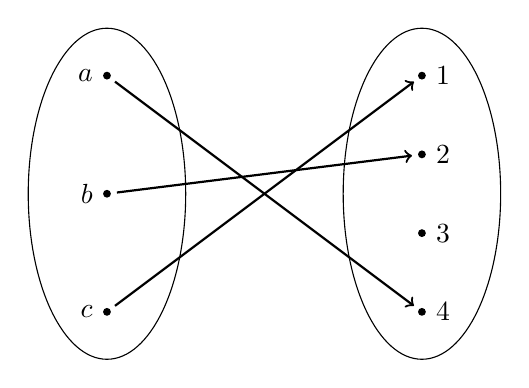
\begin{tikzpicture}[ele/.style={fill=black,circle,minimum width=.8pt,inner sep=1pt},every fit/.style={ellipse,draw,inner sep=-2pt}]
      \node[ele,label=left:$a$] (a1) at (0,4) {};    
      \node[ele,label=left:$b$] (a2) at (0,2.5) {};    
      \node[ele,label=left:$c$] (a3) at (0,1) {};
    
      \node[ele,,label=right:$1$] (b1) at (4,4) {};
      \node[ele,,label=right:$2$] (b2) at (4,3) {};
      \node[ele,,label=right:$3$] (b3) at (4,2) {};
      \node[ele,,label=right:$4$] (b4) at (4,1) {};
    
      \node[draw,fit= (a1) (a2) (a3) ,minimum width=2cm] {} ;
      \node[draw,fit= (b1) (b2) (b3) (b4),minimum width=2cm] {} ;  
      \draw[->,thick,shorten <=2pt,shorten >=2pt] (a1) -- (b4);
      \draw[->,thick,shorten <=2pt,shorten >=2] (a2) -- (b2);
      \draw[->,thick,shorten <=2pt,shorten >=2] (a3) -- (b1);

     \end{tikzpicture}
    \end{figure}
    
    Here are two ways to prove that a function is injective:
    \begin{enumerate}
        \item Consider two arbitrary distinct elements in the domain. Show that they must map to distinct outputs.
        
        \begin{mdframed}
        \begin{proof}
        Consider the function $f \vcentcolon \Z \rightarrow \mathbb{E}$ (where $\mathbb{E}$ is the set of even integers) defined by $f(x) = 2x$. Consider distinct elements $a,b \in \Z$. Assume for the sake of contradiction that $f(a) = f(b)$. Note that $f(a) = 2a$ and $f(b) = 2b$, which means $2a=2b$. But $2a \neq 2b$ since $a \neq b$. Thus, $f(a) \neq f(b)$, meaning that $f$ is injective.
        \end{proof}
        \end{mdframed}
    
        \item Consider any arbitrary two equal elements in the image of $f$ (say, $f(a)$ and $f(b)$). Show that $a = b$.
        
        \begin{mdframed}
        \begin{proof}
        Consider the function $f \vcentcolon \Z \rightarrow \mathbb{E}$ defined by $f(x) = 2x$. Consider $f(a)$ and $f(b)$ in the image of $f$, where $f(a) = f(b)$. Note that $f(a) = 2a$ and $f(b) = 2b$. Thus, $2a = 2b$, meaning that $a = b$, proving injectivity.
        \end{proof}
        \end{mdframed}
    \end{enumerate}
    
    \subsection{Surjectivity}
    A function is surjective if, for all $b \in B$, there exists at \textit{least} one $a \in A$ such that $f(a) = b$. In other words, no element in the co-domain gets left behind: there is always some element that maps to it. Equivalently, a function is surjective if the image of the function is the entire co-domain.
    
    If a function $f \vcentcolon A \rightarrow B$ is surjective, we know that $|A| \geq |B|$ because every element in $B$ needs some element in $A$ to map to it, so $A$ needs to have at least as many elements as $B$.
    
    \begin{figure}[h]
     \centering
     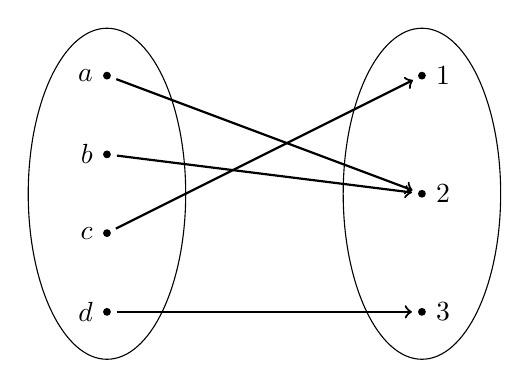
\begin{tikzpicture}[ele/.style={fill=black,circle,minimum width=.8pt,inner sep=1pt},every fit/.style={ellipse,draw,inner sep=-2pt}]
      \node[ele,label=left:$a$] (a1) at (0,4) {};    
      \node[ele,label=left:$b$] (a2) at (0,3) {};    
      \node[ele,label=left:$c$] (a3) at (0,2) {};
      \node[ele,label=left:$d$] (a4) at (0,1) {};
    
      \node[ele,,label=right:$1$] (b1) at (4,4) {};
      \node[ele,,label=right:$2$] (b2) at (4,2.5) {};
      \node[ele,,label=right:$3$] (b3) at (4,1) {};
    
      \node[draw,fit= (a1) (a2) (a3) (a4),minimum width=2cm] {} ;
      \node[draw,fit= (b1) (b2) (b3) ,minimum width=2cm] {} ;  
      \draw[->,thick,shorten <=2pt,shorten >=2pt] (a1) -- (b2);
      \draw[->,thick,shorten <=2pt,shorten >=2] (a2) -- (b2);
      \draw[->,thick,shorten <=2pt,shorten >=2] (a3) -- (b1);
      \draw[->,thick,shorten <=2pt,shorten >=2] (a4) -- (b3);
     \end{tikzpicture}
    \end{figure}
    
    To prove that a function is surjective, consider an arbitrary element in the co-domain, and construct a specific element in the domain that maps to it.
    
    \begin{mdframed}
    \begin{proof}
    Consider the function $f \vcentcolon \Z \rightarrow \mathbb{E}$ defined by $f(x) = 2x$. Consider an arbitrary element in the co-domain $b$. Since $b$ is even, $b = 2a$ for some $a \in \Z$. By definition of $f$, $f(a) = 2a = b$, and so we've found the element that maps to $b$, proving surjectivity.
    \end{proof}
    \end{mdframed}
    
    \subsection{Bijectivity}
    
    A bijection is a function that is both injective and surjective. Thus, to prove that a function is a bijection, prove that it is injective and surjective.
    
    If we combine our results from injectivity and surjectivity, we know that the cardinality of the domain must be less than or equal to that of the co-domain (by injectivity), and that the cardinality of the domain must be greater than or equal to that of the domain (by surjectivity.) Thus, the cardinalities of the two sets must be equal.
    
    \begin{center}
    \textit{There exists a bijection between two sets if and only if they have equal cardinality.}
    \end{center}
    
    Thus, to prove that the sizes of two sets are equal, it suffices to prove that there exists a biejction between them.

        
    \begin{figure}[h]
     \centering
     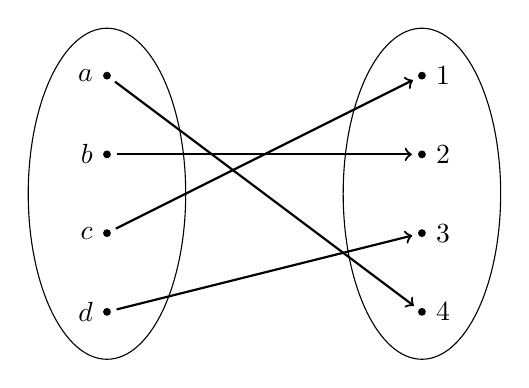
\begin{tikzpicture}[ele/.style={fill=black,circle,minimum width=.8pt,inner sep=1pt},every fit/.style={ellipse,draw,inner sep=-2pt}]
      \node[ele,label=left:$a$] (a1) at (0,4) {};    
      \node[ele,label=left:$b$] (a2) at (0,3) {};    
      \node[ele,label=left:$c$] (a3) at (0,2) {};
      \node[ele,label=left:$d$] (a4) at (0,1) {};
    
      \node[ele,,label=right:$1$] (b1) at (4,4) {};
      \node[ele,,label=right:$2$] (b2) at (4,3) {};
      \node[ele,,label=right:$3$] (b3) at (4,2) {};
      \node[ele,,label=right:$4$] (b4) at (4,1) {};
    
      \node[draw,fit= (a1) (a2) (a3) (a4),minimum width=2cm] {} ;
      \node[draw,fit= (b1) (b2) (b3) (b4),minimum width=2cm] {} ;  
      \draw[->,thick,shorten <=2pt,shorten >=2pt] (a1) -- (b4);
      \draw[->,thick,shorten <=2pt,shorten >=2] (a2) -- (b2);
      \draw[->,thick,shorten <=2pt,shorten >=2] (a3) -- (b1);
      \draw[->,thick,shorten <=2pt,shorten >=2] (a4) -- (b3);
     \end{tikzpicture}
    \end{figure}
    
\subsection{Intuition and Examples}
\begin{mdframed}
For each of the following, state if it is a function, injections, surjection, or neither.
\begin{enumerate}[(a)]
    \item $f : \Z \rightarrow \Z$ where $f(x) = x^2$
    
    A function but not injective or surjective.
    
    \item $f : \Z^+ \rightarrow \Z^+$ where $f(x) = x^2$. $\Z^+$ denotes the positive integers.
    
    Function, Injection.
    \item $f: \Z \rightarrow \Z$ where $f(x) = \sqrt{x}$.
    
    Not a function.
    \item $f : \text{First Year Students at Brown} \rightarrow \text{First Year Dorms at Brown}$ where $f(\text{student}) = $ the dorm that the student lives in.
    
    Function, Surjection.
    \item $f : \text{Students at Brown} \rightarrow \text{Banner IDs of current Students}$ where $f(\text{student}) = $ the banner ID of student.
    
    Function, Bijection.
    
    \item $f : \text{People in the World} \rightarrow  \{0,1\}$ where $f(\text{person}) = $ 1 if they are Prof. Littman and 0 otherwise.
    
    Function, Surjection.
    
    \item $f : \text{Library at Brown} \rightarrow \Z$ where $f(\text{Library}) = $ number of books in the library.
    
    Function, Injection.
    
    \item $f: S \rightarrow \Pow{(S)}$ where $f(S) = \{S\}$.
    
    Function, Injection.
    
    \item $f: \Pow{(\{1,2,4\})} \rightarrow \{0,1,2,3\}$ where $f(X) = |X|$.
    
    Fucntion, Surjection.
\end{enumerate}
\end{mdframed}
    
\section{Induction}

We next review mathematical induction.

\subsection{Example 1: Template and Weak Induction}

\idea \textit{If you are stuck on an induction problem on the exam, start by writing out the inductive hypothesis and the structure of the proof. You will receive partial credit for doing so and it may also help you think of how to proceed.}

\idea \textit{Often the inductive step is a direct proof using the inductive hypothesis. It is not always the case, sometimes you might have to use \textbf{different cases} or even \textbf{contradiction}.}

\begin{mdframed}
We will first provide a review of the template for an inductive proof and provide an example.

      For example, say we are trying to prove that $\sum_{i=0}^n i = \frac{n(n+1)}{2}$ is true for all $n \in \mathbb{N}$. 

      \begin{enumerate}
        \item Define the predicate $P(n)$.

        \textit{Let $P(n)$ be the predicate that $\sum_{i=0}^n i = \frac{n(n+1)}{2}$.}

        \item Show that the base case is true.

        \textit{We will first show $P(0)$ is true. $\sum_{i=0}^0 i = 0$ and $\frac{0(0+1)}{2} = 0$ so they are equal as needed.}

        \item Assume the inductive hypothesis is true. If you are using stardard induction, then you will assume 
			$P(k)$ is true for some integer $k$. If you are using strong induction then you will assume $P(i)$ is true for all $i \leq k$. Either way, you should specify that $k$ is some integer greater than or equal to your greatest base case.

        \textit{Assume $P(k)$ is true for some arbitrary integer $k \geq 0$.}

        \item Show that $P(k+1)$ is true given the inductive hypothesis.

		\textit{We will now show that  $\sum_{i=0}^{k+1} i = \frac{(k+1)(k+2)}{2}$}.

       	\textit{We know that $\sum_{i=0}^{k+1} i = \left( \sum_{i=0}^{k} i \right)+ (k+1)$.}

		\textit{By our inductive hypothesis $\sum_{i=0}^k i = \frac{k(k+1)}{2}$.}

         \textit{Therefore,}
		\begin{align*}
			\sum_{i=0}^{k+1} i &= \left( \sum_{i=0}^{k} i \right)+ (k+1) \\
			&=  \frac{k(k+1)}{2} + (k+1) \\
			&= \frac{k(k+1) + 2(k+1)}{2} \\
			&= \frac{(k+1)(k+2)}{2}
		\end{align*}
		\textit{as needed.}\qed

        \item Conclude the proof.
        
        \textit{Therefore, as $P(0)$ is true and $P(k)$ implies $P(k+1)$ for all $k \in \Z$, $k \geq 0$, $P(n)$ is true for all nonnegative integers $n$.}
      \end{enumerate}
\end{mdframed}

\subsection{Example 2: Strong Induction}
\begin{mdframed} Define the sequence $S$ as follows: $S_1 = 1$, $S_2 = 3$, $S_n = S_{n-1} * S_{n-2}$ for integers $n \geq 2$. Prove that $S_n$ is odd for all positive integers $n$.

\begin{proof} Let $P(n)$ be the predicate that $S_n$ is odd.

\textbf{Base Cases:} $S_1 = 1$ and $S_2 = 3$, which are both odd, so $P(1)$ and $P(2)$ are both true.

\textbf{Inductive Hypothesis:} For some arbitrary integer $k \geq 2$, assume for all positive integers $i \leq k$ that $P(i)$ is true. That is, assume $S_1$ through $S_k$ are odd.

\textbf{Inductive Step:} Consider $S_{k+1}$. As $k \geq 2$, $S_{k+1} = S_k * S_{k-1}$. By the inductive hypothesis, $S_k$ and $S_{k-1}$ are both odd. As we proved in Section~2.1, the product of two odd numbers is odd, so $S_{k+1}$ is odd. Therefore, $P(k+1)$ is true.

\textbf{Conclusion:} Thus, as $P(1)$ and $P(2)$ are true and, for any positive integer $k$, $P(1)$,...,$P(k)$ imply $P(k+1)$, $P(n)$ is true for all positive integers $n$; all terms in the sequence are odd.
\end{proof}
\end{mdframed}

\end{document}
